\chapter{System design}
\label{chap:systdesign}
This chapter describes the technical aspects of the design of \projectname.

\section{Design method}
\label{sec:designMethod}
\projectname{} is implemented as a web application using the Java software development framework Google Web Toolkit (GWT). Section \ref{sec:decompdescr} defines the components of \projectname{} and their dependencies.


\section{Decomposition description}
\label{sec:decompdescr}
The decomposition of \projectname\ into components is based on the requirements of the URD \cite{urd} and the SRD \cite{srd}.

\fpstartparagraph{} Section \ref{subsec:complist} lists the components, which are further described in chapter \ref{chap:compdescr}. Section \ref{subsec:depdiag} illustrates the dependencies between the components. The identified components are strongly based on the tiers listed in section \ref*{SRD-sec:moddesc} of the SRD \cite{srd}. An overview of these tiers is given in Figure  \ref*{SRD-fig:tierchannel} of the SRD \cite{srd}.

\subsection{List of components}
\label{subsec:complist}
The following components are identified:

\begin{itemize}
	\item Server
	\begin{itemize}
		\item Application Persistence
		\item HTTP Server
		\item Fortran Module
		\item Application Service
		\item Simulator Service
	\end{itemize}

\newpage

	\item Client
	\begin{itemize}
		\item Client Browser
	\begin{itemize}
		\item Layout
		\item Application State
	\end{itemize}
		\item Client Persistence
	\end{itemize}
\end{itemize}

\subsection{Dependencies diagram}
\label{subsec:depdiag}

Figure \ref{fig:compdependencies} illustrates the dependencies between the components of \projectname{}. Arrows indicate a `depends on' relation between components. This relationship means that the component on the start of the arrow needs the functionality of the component on the end of the arrow to fulfill its task. A double arrow indicates a bidirectional relationship, so the components on both sides of the arrow need eachother.

\noindent
\begin{figure}[h!b]
	\centering
	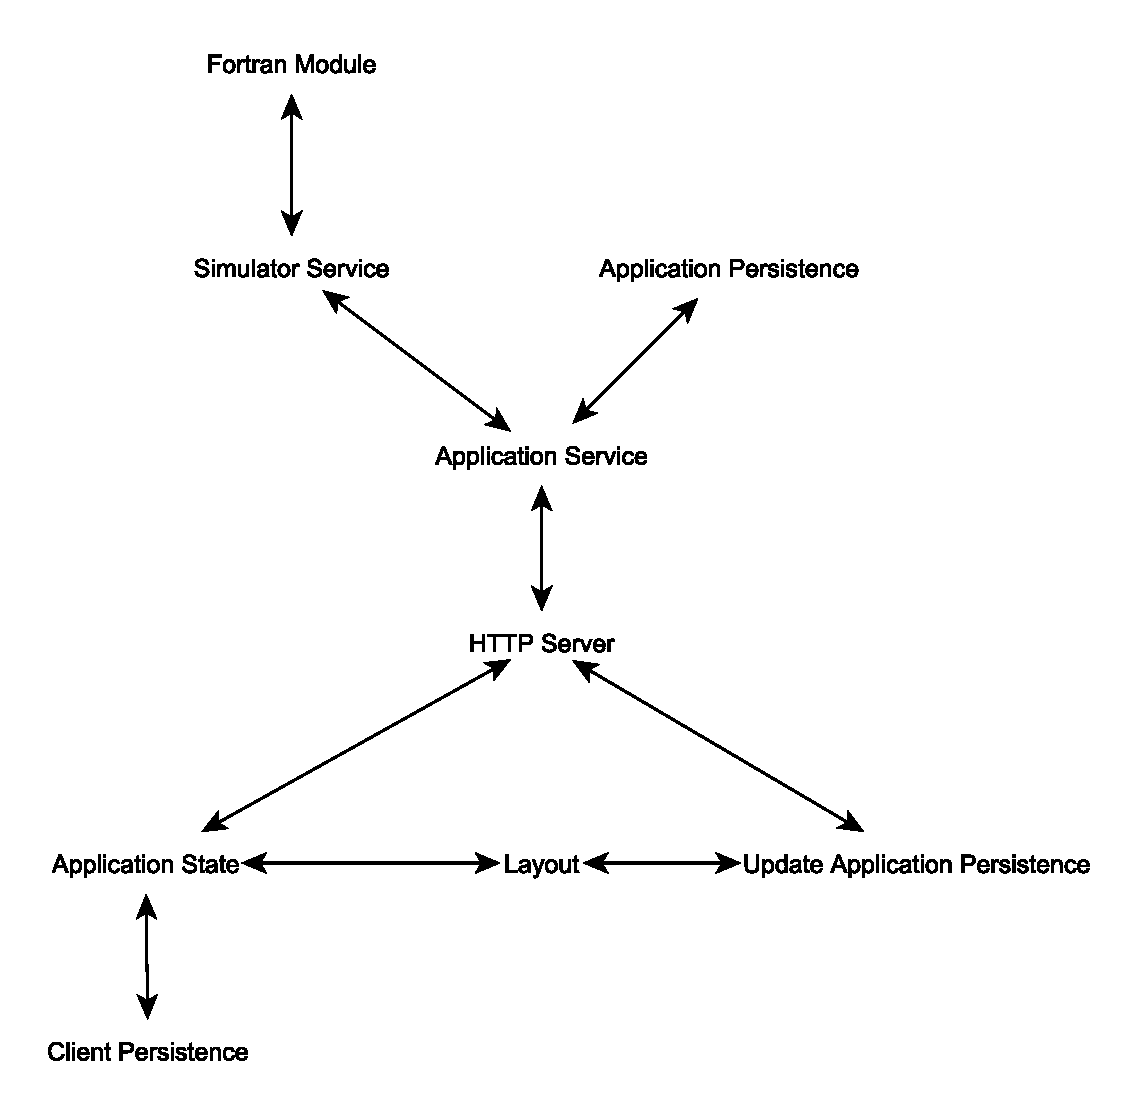
\includegraphics[width=\textwidth]{ComponentDependencies}
	\caption{Components of \projectname\ and their dependencies}
	\label{fig:compdependencies}
\end{figure}
